\begin{figure*}[t]
\centering
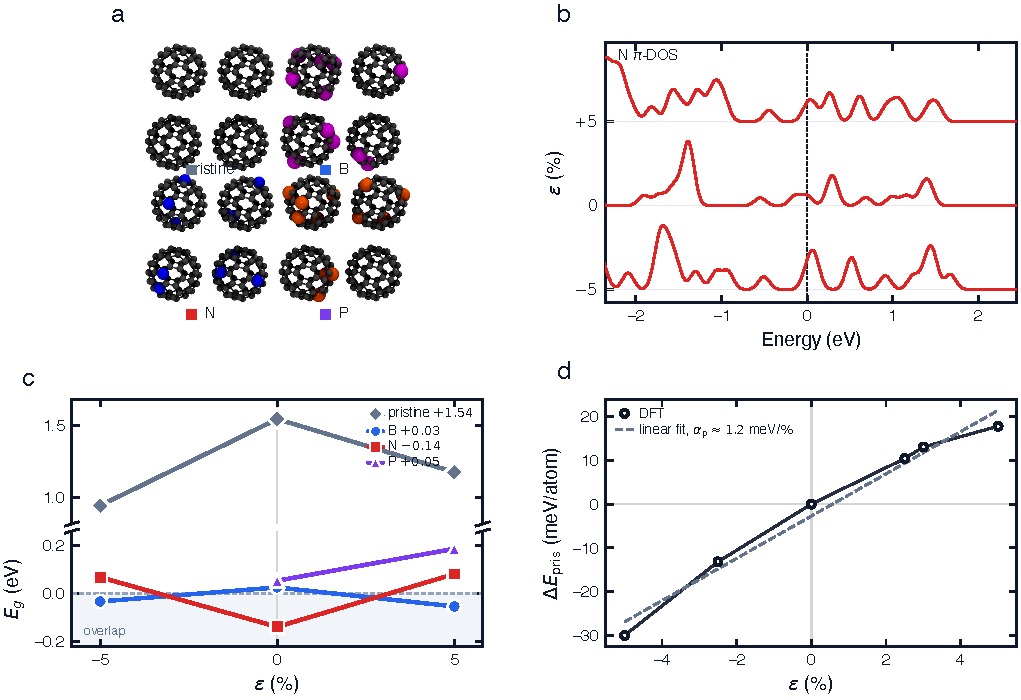
\includegraphics[width=\textwidth]{figures/out/figure_prb_1_electronic.pdf}
\caption{\label{fig:electronic}Reference tetramer and one-parameter strain slices (PBE+D3).
(a)~qHP C$_{60}$ tetramers at $\epsilon{=}0$: pristine (top left), B (top right), N (bottom left), P (bottom right), with substituent sites highlighted (covalent-radius excess in Table~\ref{tab:geometry}). Heteroatoms and the key below the mosaic use CPK colors, which differ from the trajectory palette of panels (c) and (d).
(b)~N $\pi$-DOS vs.\ energy, stacked by biaxial strain $E_{\mathrm{F}}{=}0$.
(c)~Frontier HOMO--LUMO separation $E_{\mathrm{H-L}}(\epsilon)$ from the archived $\pi$-DOS spectra. Pristine keeps a $1.0$--$1.5$~eV gap; all three substituted cages close it to $|E_{\mathrm{H-L}}|\lesssim 0.2$~eV, and the residual separation changes sign with strain because the frontier levels cross---a gap-closure indicator, not a negative gap. PBE underestimates gaps, so only the pristine-vs.-substituted contrast is interpreted.
(d)~Pristine mechanical $\Delta E(\epsilon)$ and linear $\alpha$.
Joint-load four-corner audits are in Fig.~\ref{fig:synergy}.}
\end{figure*}
